\section{zadanie 6}
Zadanie polegało na przeprawadzeniu eksperymentów dla funkcji rekurencyjnej:
\[ x_{n+1} := x_n^2+c, \textrm{dla } n = 0,1,2,...\]
dla danych początkowych:
\begin{itemize}
  \item \textbf{Test 1}: \(c = -2, x_0 = 1\)
  \item \textbf{Test 2}: \(c = -2, x_0 = 2\)
  \item \textbf{Test 3}: \(c = -2, x_0 = 1.99999999999999\)
  \item \textbf{Test 4}: \(c = -1, x_0 = 1\)
  \item \textbf{Test 5}: \(c = -1, x_0 = -1\)
  \item \textbf{Test 6}: \(c = -1, x_0 = 0.75\)
  \item \textbf{Test 7}: \(c = -1, x_0 = 0.25\)
\end{itemize}
Dla danych początkowych program wykonywał 40 iteracji.
\subsection{Wyniki:}

\begin{figure}[ht]
  \centering
  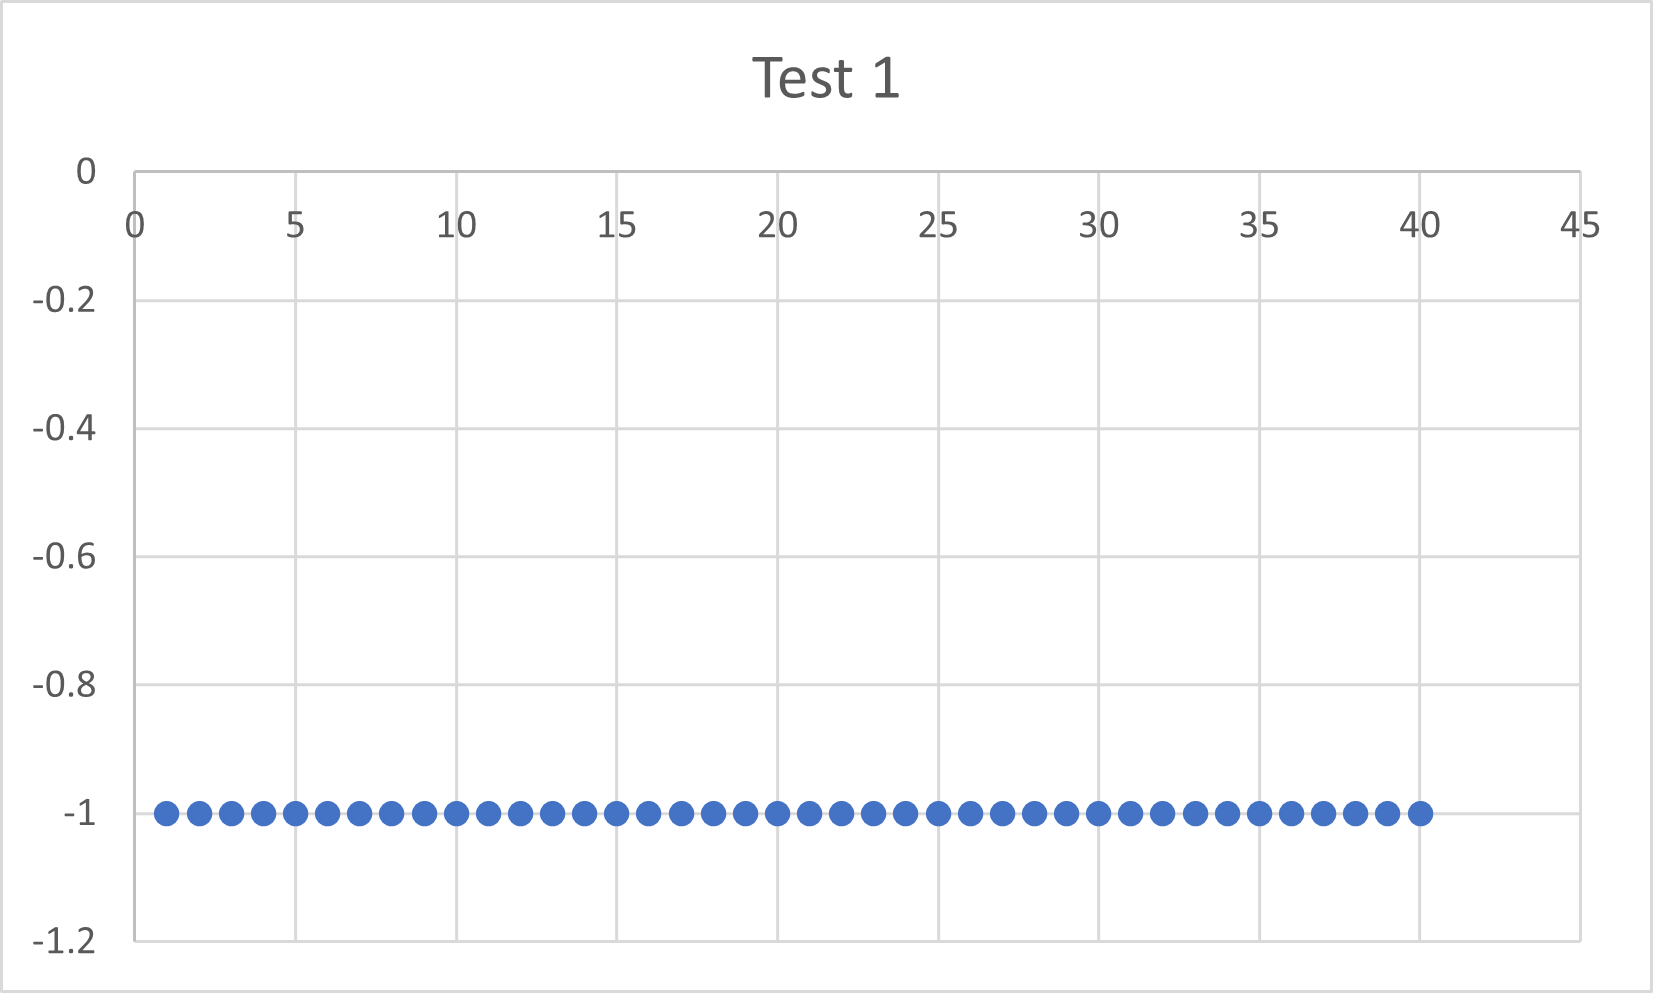
\includegraphics[width=\textwidth]{zadanie 6/test 1.png}
  \caption{Test 1}
  \label{fig:test1}
\end{figure}
\begin{figure}[ht]
  \centering
  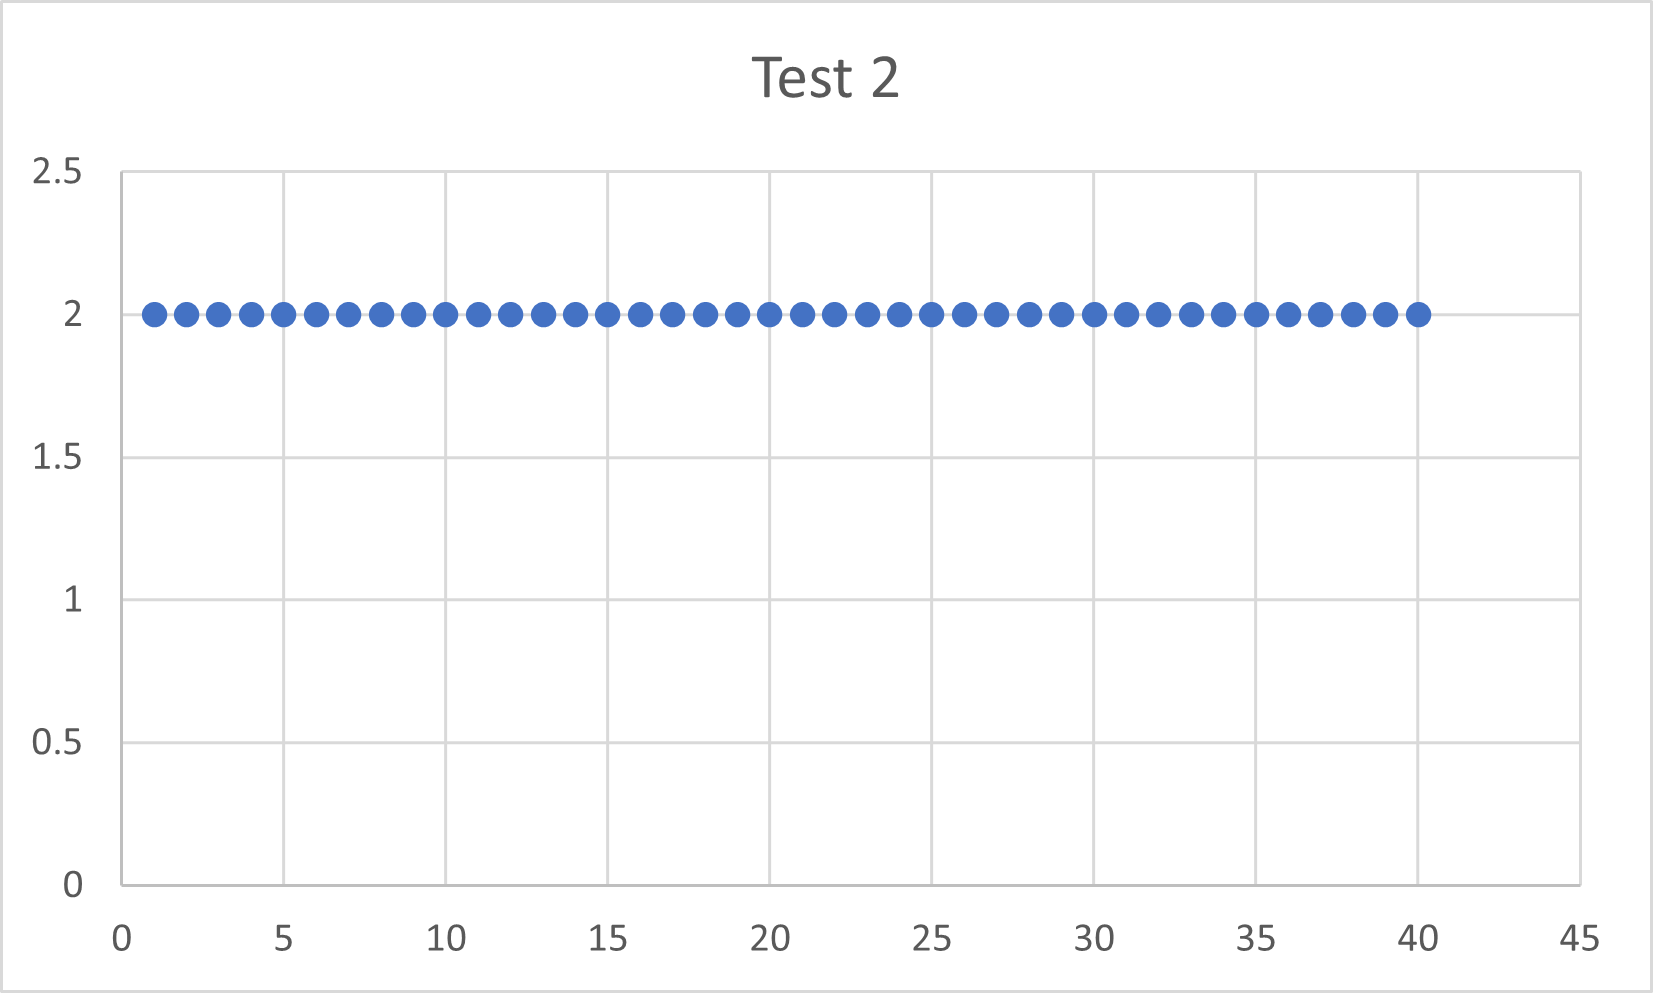
\includegraphics[width=\textwidth]{zadanie 6/test 2.png}
  \caption{Test 2}
  \label{fig:test2}
\end{figure}
\begin{figure}[ht]
  \centering
  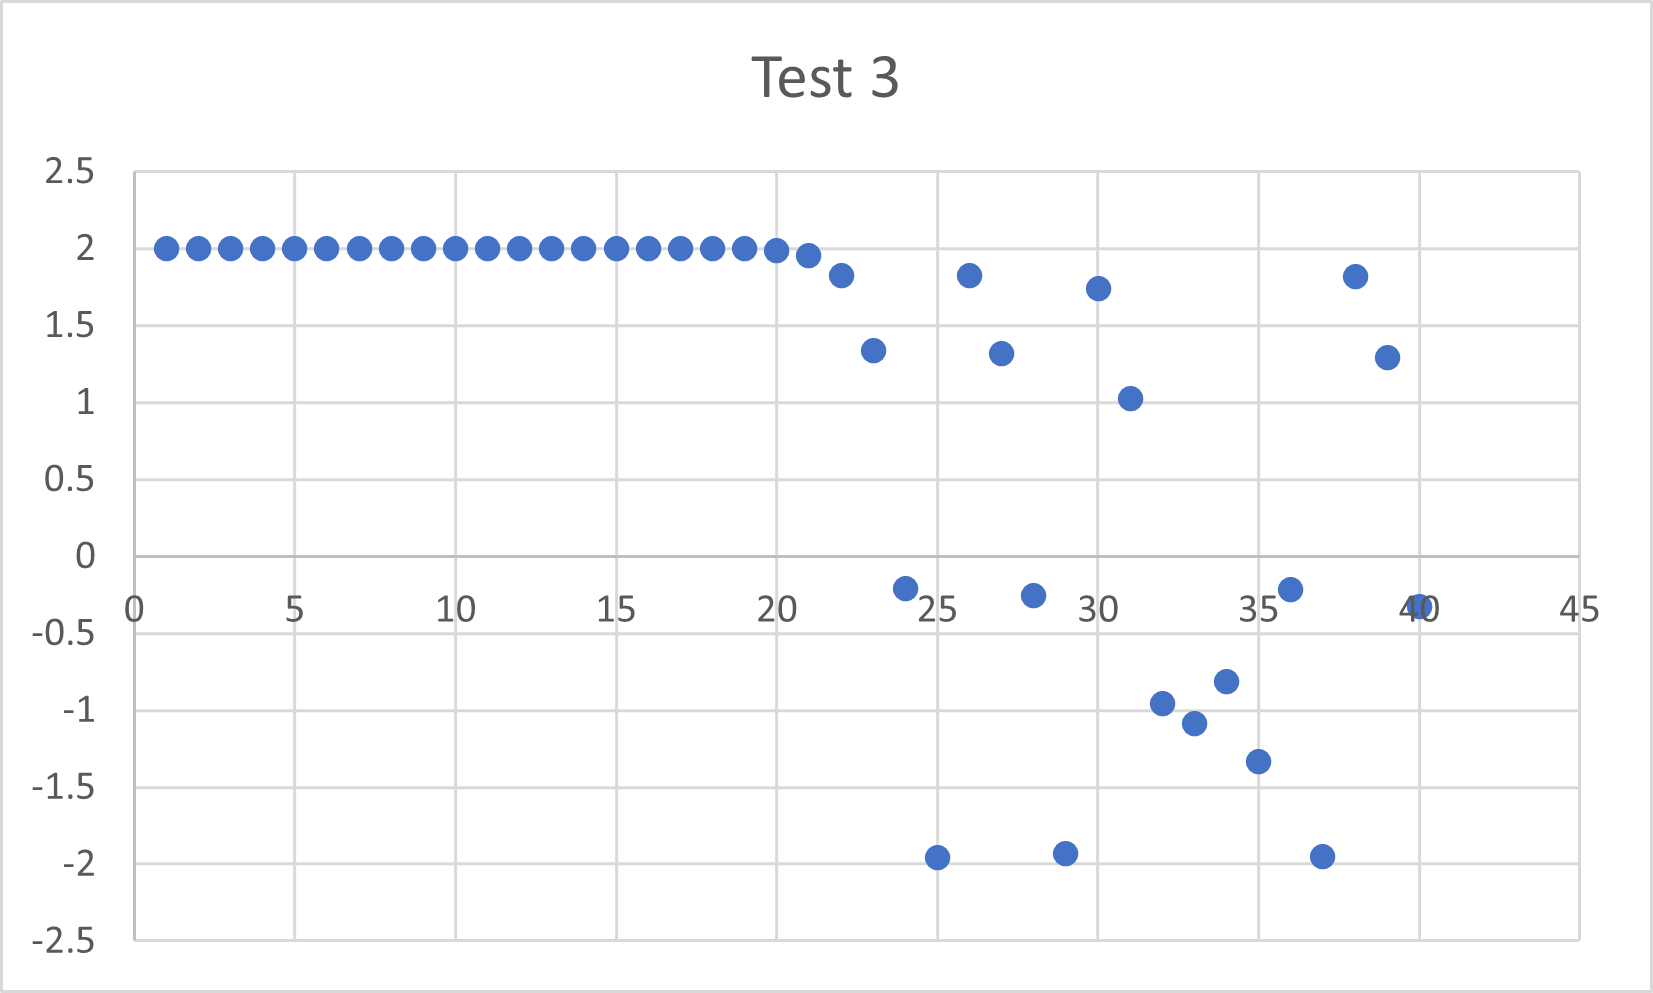
\includegraphics[width=\textwidth]{zadanie 6/test 3.png}
  \caption{Test 3}
  \label{fig:test3}
\end{figure}
\begin{figure}[ht]
  \centering
  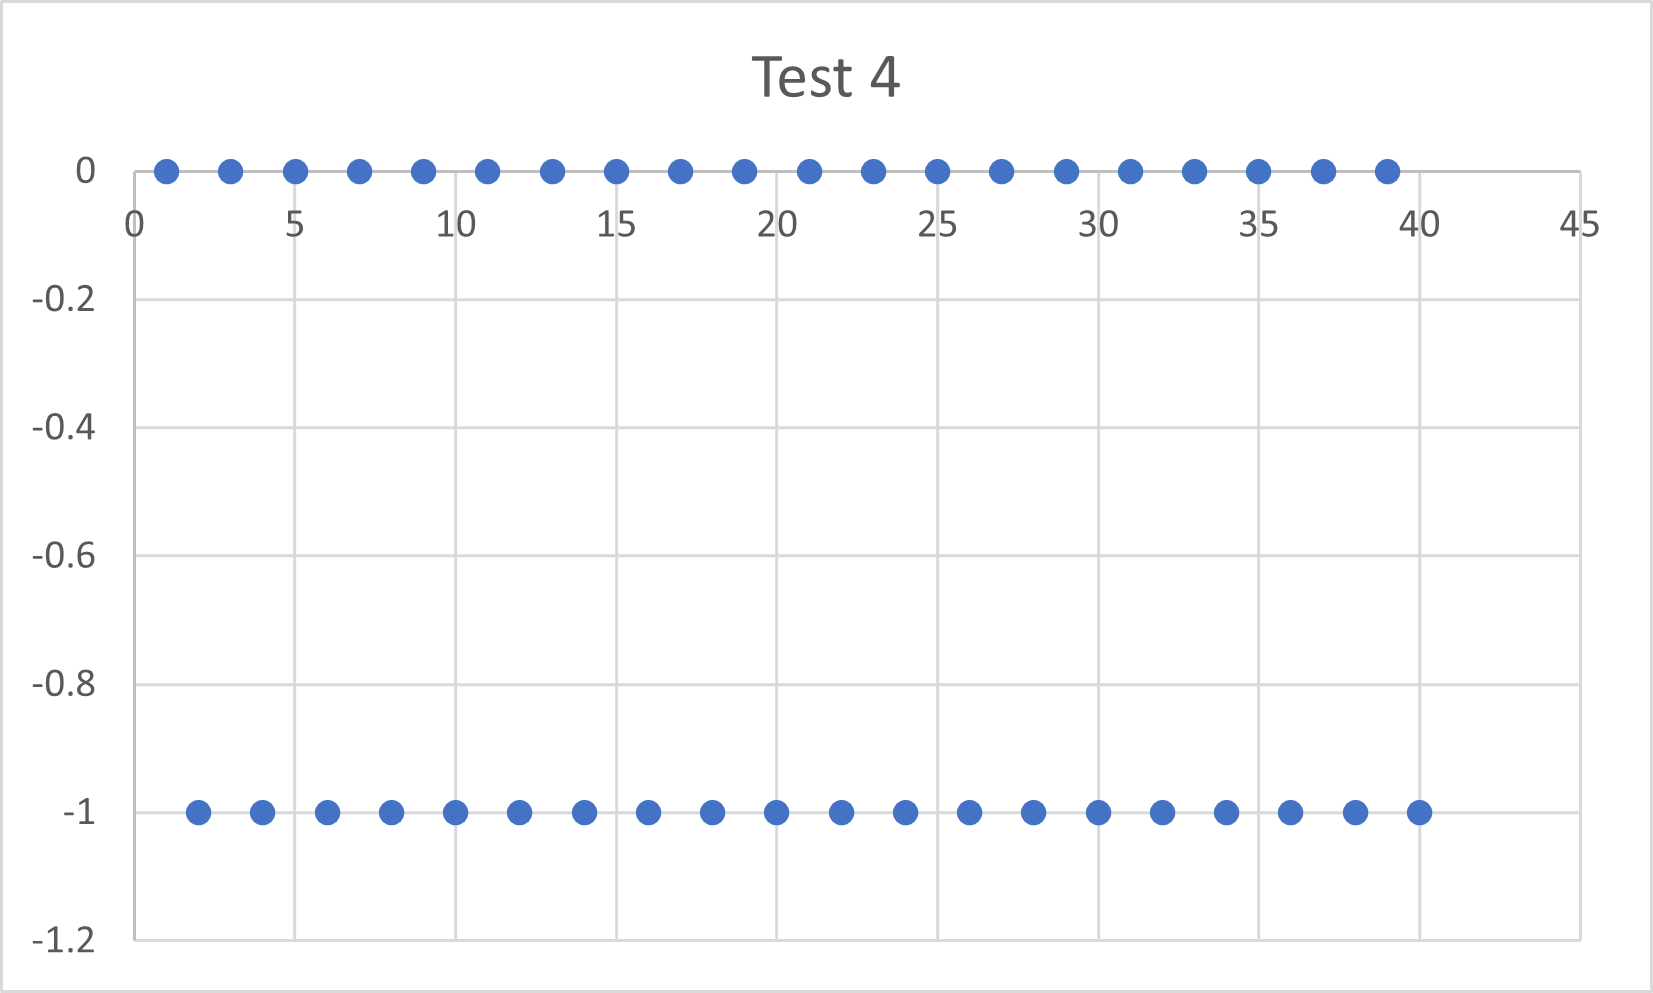
\includegraphics[width=\textwidth]{zadanie 6/test 4.png}
  \caption{Test 4}
  \label{fig:test4}
\end{figure}
\begin{figure}[ht]
  \centering
  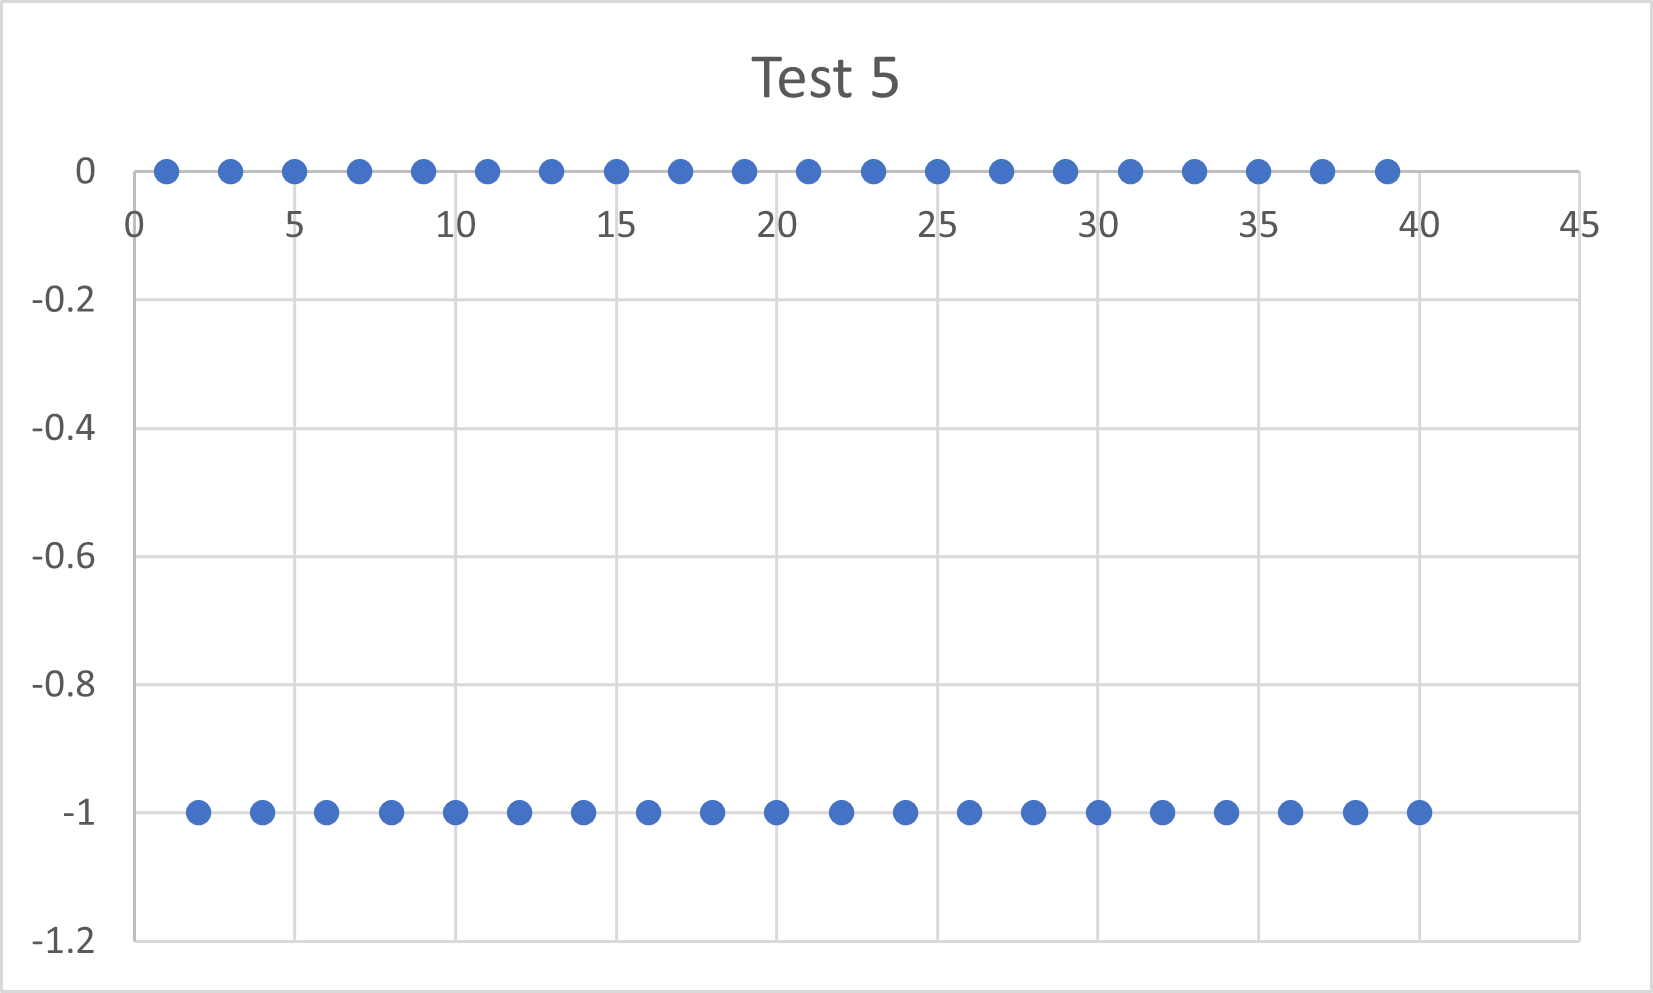
\includegraphics[width=\textwidth]{zadanie 6/test 5.png}
  \caption{Test 5}
  \label{fig:test5}
\end{figure}
\begin{figure}[ht]
  \centering
  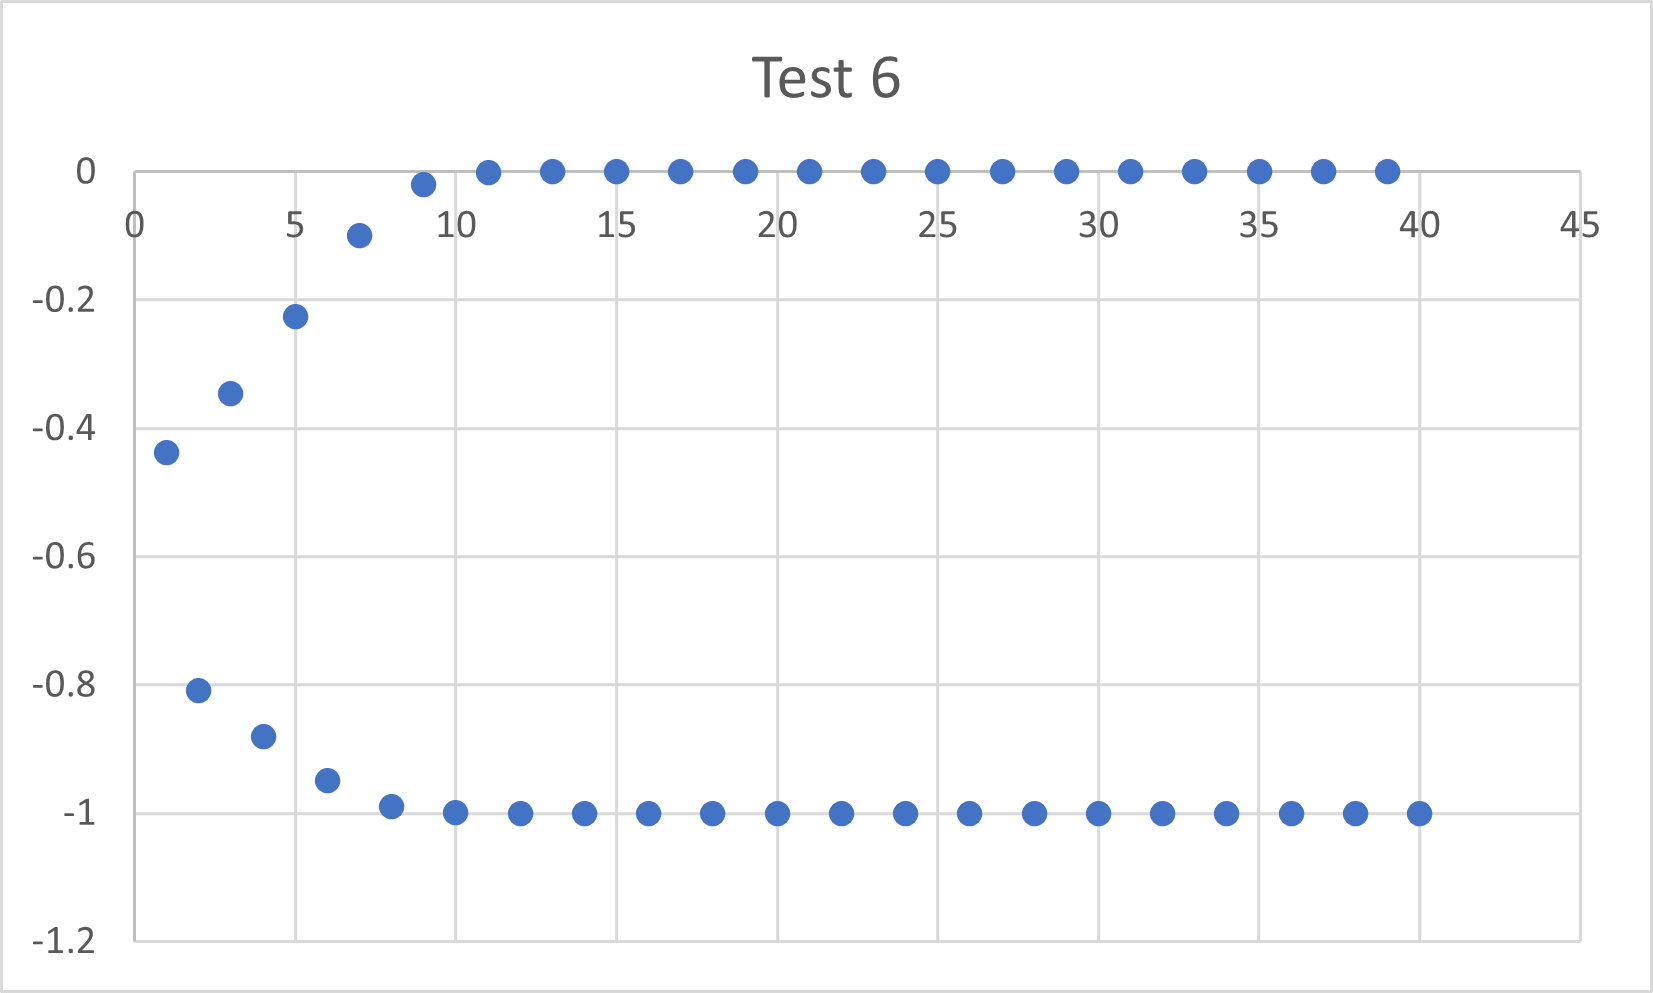
\includegraphics[width=\textwidth]{zadanie 6/test 6.png}
  \caption{Test 6}
  \label{fig:test6}
\end{figure}
\begin{figure}[ht]
  \centering
  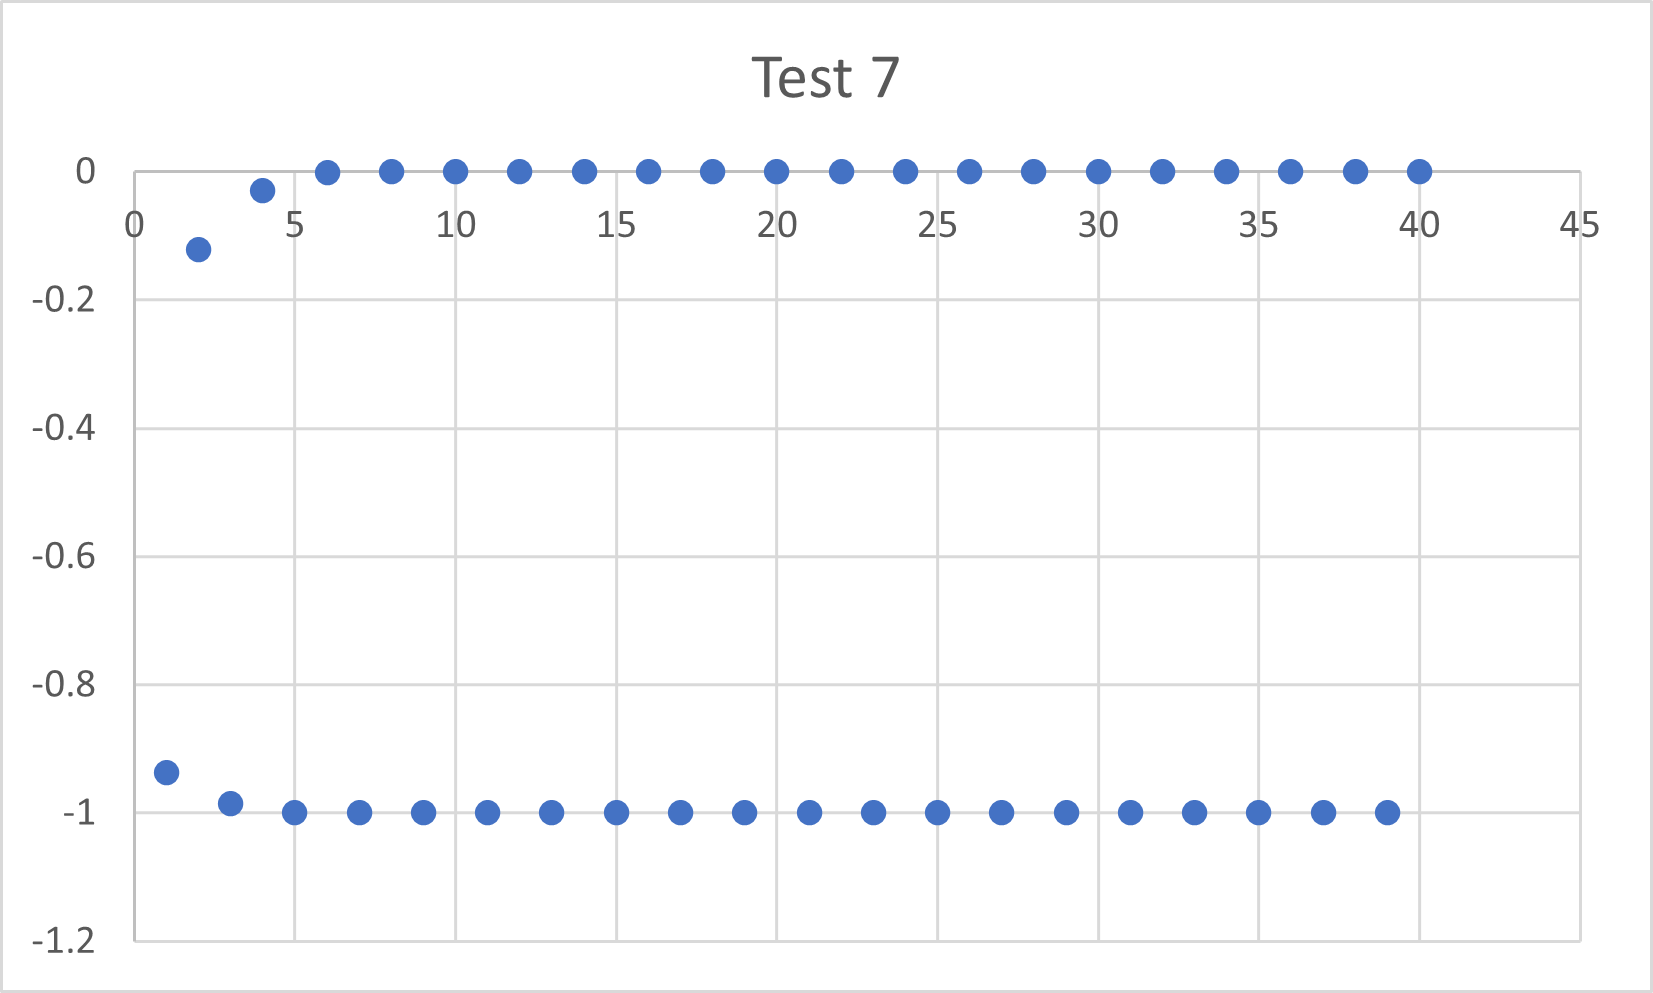
\includegraphics[width=\textwidth]{zadanie 6/test 7.png}
  \caption{Test 7}
  \label{fig:test7}
\end{figure}

\subsection{Wnioski:}
Dla testów 2 i 3 dla niewielkiej zmiany danych wejściowych dane wyjściowe mają duży rozrzut. Z kolei dla różnych danych wejściowych eksperymentów 4 i 5 dane wyjściowe zachowują się identycznie. Wykresy 6 i 7 również wykazują pewne podobieństwo mimo że różnica danych wejściowych jest znaczna.

